\chapter{State of the Art} \label{chap:sota}

\section*{}

This chapter starts with an overview of online marketing in the last few years, followed by a review of the data mining algorithms that can be used to solve the same kind of problems as this thesis.

\section{Online Advertising Overview}

Before entering in details about the state of the art of the technologies that can be used to
help solve the presented problem, it is better to explain some basic concepts about the world of online advertising.

All advertising has the main purpose of getting a message to the people that will impact or influence them in some way,
therefore the same goal is applied to online advertising.
One of the metrics of advertising are impressions, which correspond to the number of times a user sees the message (the ad).\cite{kOA}
\textbf{Ads} can present itself in various sizes\cite{kOA2}, forms and locations \cite{kOA3}, and these characteristics are chosen both by the advertiser
and the publisher to better serve their purpose.
\textbf{Campaigns} are composed by two big parts, which are the ads that compose it and the target population that they pretend to reach,
including the rules of this targeting. For example, \textbf{frequency capping} to limit the number of times the same advertising is shown to the user \cite{kOA},
avoiding, in this way, showing the same ad multiple times in a row to the same user, that can lead to a bad response from his part.\cite{Buchbinder20141}

Nowadays, the main pricing models of online advertising are:
\begin{itemize}
\item\textbf{Cost-per-Mile} where the advertiser pays per impression. The main problem of this model is the advertiser as to pay to the publisher even
if the ad doesn't lead to any profit.
\item\textbf{Cost-per-Click} where the advertiser pays per click to the publisher. This model is more expensive per unit\cite{Performics}, but on overall can be more
profitable\cite{Performics} if the audience of the websites where the ad is imprinted is more interested in that kind of product/service\cite{Andrea2004}.
\item\textbf{Cost-per-lead} where the advertiser pays for a lead. If this model is being used the advertiser doesn't pay per number of impressions nor per clicks. Instead, pays only
if he gets valid information about the user, like the information of a sign up form for a community.
\item\textbf{Cost-per-Action} or \textbf{Cost-per-Order} where the advertiser is charged per buy or action. This model is similar to CPL but has in mind an instantaneous return of
the investment.
\end{itemize}

Traditionally, publishers sell their space to advertisers in bulk (\textbf{Ad networks}) this method has its \textit{ups} and \textit{downs}.
The obvious \textit{up} is that sometimes the advertiser gets premium spots at low prices.
On the other hand, one of the biggest drawbacks is that when the advertiser buys the impressions as a
closed package, sometimes impressions are not maximized in terms of profit.
Other problem of traditional methods that, although the \emph{CPA} and \emph{CPL} pricing methods minimize the risk for the advertiser, the responsibility of
optimizing conversion rate\footnote{ See, e.g., \url{http://www.marketingterms.com/dictionary/conversion_rate/}} is still
on the ad network hands.\cite{Yuan:2013:RBO:2501040.2501980}

In the past few years, a new model called \textbf{Real Time Bidding}\index{Real Time Bidding}\index{RTB} has been gaining terrain \cite{Adfonic}.
\emph{RTB}, as the name gives, is a market where publishers offer his advertisement space and advertisers bid over it in real time. This allow publishers to get
the best value for their space and advertisers get the best placement for their advertisement.

There are three main players in the world of \emph{RTB}\index{Real Time Bidding}:
\begin{itemize}
\item The \textbf{Demand Side Platform}\index{DSP} is a tool used by the advertisers to act on their behalf on the \emph{RTB}. \emph{DSPs}\index{DSP} allows them to set
their campaigns' parameters and to monitor the performance of the campaign. This way the advertisers try to get the best performance of their campaigns because 
\emph{DSPs} use algorithms driven by performance data.\cite{Gern201230}
\item The \textbf{Publisher} provides the inventory, that is comprised by accesses made by users. In some cases, the publisher uses \textbf{Supply Side Platforms}.
\emph{SSPs} help the publisher to better manage his inventory, and even let him set a reserve price for their inventory.\cite{Yuan:2013:RBO:2501040.2501980}
\item The \textbf{Ad Exchange} looks a little like a stock exchange, but in reality is a software platform that mediates the exchange. This exchange takes place in
a few milliseconds while the page loads.
\end{itemize}

\emph{RTB} allows some features of paid search advertising everywhere \cite{Gern201230}, because it allows the advertiser to better select
the inventory\footnote{ this inventory is made of user accesses} where he wants their campaigns to run on.
The flexibility that \emph{RTB} gives to all the intervinients of this exchange is what demands the necessity of predicting the future inventory, to
better access its value.



\section{Data Mining}\label{sec:datamining}
%\begin{quote}
''Data mining is about solving problems by analyzing data already present in databases.''\cite[p. 5]{Witten:2005:DMP:1205860}
%\end{quote}
. Furthermore, consists in a vast number of techniques used to find interesting patterns in large datasets and translate
that huge quantity of raw data in information and/or knowledge. 

Data mining uses techniques from various fields, mostly from mathematics and computer science,
such as artificial intelligence, machine learning and statistics.
Data mining is sometimes referred as the natural evolution of information technologies \cite[p. 1]{HanKam06}

There are lots of methods of data mining, which can be separated in two groups: descriptive data mining and predictive
data mining \cite{Fayyad96knowledgediscovery}.
The main focus of the first group is to find the underlying structure of a given dataset, which methods try to find relationships and connections
between the values, without have the goal of predicting the future. On the other hand,
predictive data mining goal is to predict explicit values from patterns found on the original data set. These methods are used to build models based on past
events that can be used to predict future events.
This division is not always sharp and in some cases an algorithm mixes the two methods (predictive \& descriptive)\cite{Fayyad96knowledgediscovery}.

According to previous statements it is easy to notice that data mining doesn't apply only to one set of problems and can be used to solve many different types of
problems. The most common methods are:
\begin{itemize}
\item \textbf{Anomaly Detection} tries to discover abnormal data on the dataset. This can be useful for identifying suspicious activity on a bank
account log for example.
\item \textbf{Classification} is a method to identify which of a given set of categories a new observation belongs.
\item \textbf{Clustering} is the method of grouping similar data together, in a finite number of categories, without prior knowledge of
the characteristics of each group or the data.
\item \textbf{Dependency modeling} tries to find associations between variables. For example, trying to find out which clothes go well together.
\item \textbf{Summarization} is a method to provide an overview of the dataset, sometimes including visual representation and/or report generation.
\item \textbf{Regression} tries to find a function that can represent a given dataset with the least error associated.
\end{itemize}

\subsection{Classification Algorithms}\label{sec:classification}

\subsubsection{Decision Trees}

Decision trees algorithms use a decision tree as a predictive model where all internal nodes (non-leaf nodes) are a test for the value of an attribute that will
ultimately lead to a leaf node with the class attribute value (see example in figure~\ref{fig:dtree}).
In other words, the selection of the class value is only based on the attribute values of the entry.\cite{HanKam06}

\begin{figure}[h]
  \begin{center}
    \leavevmode
    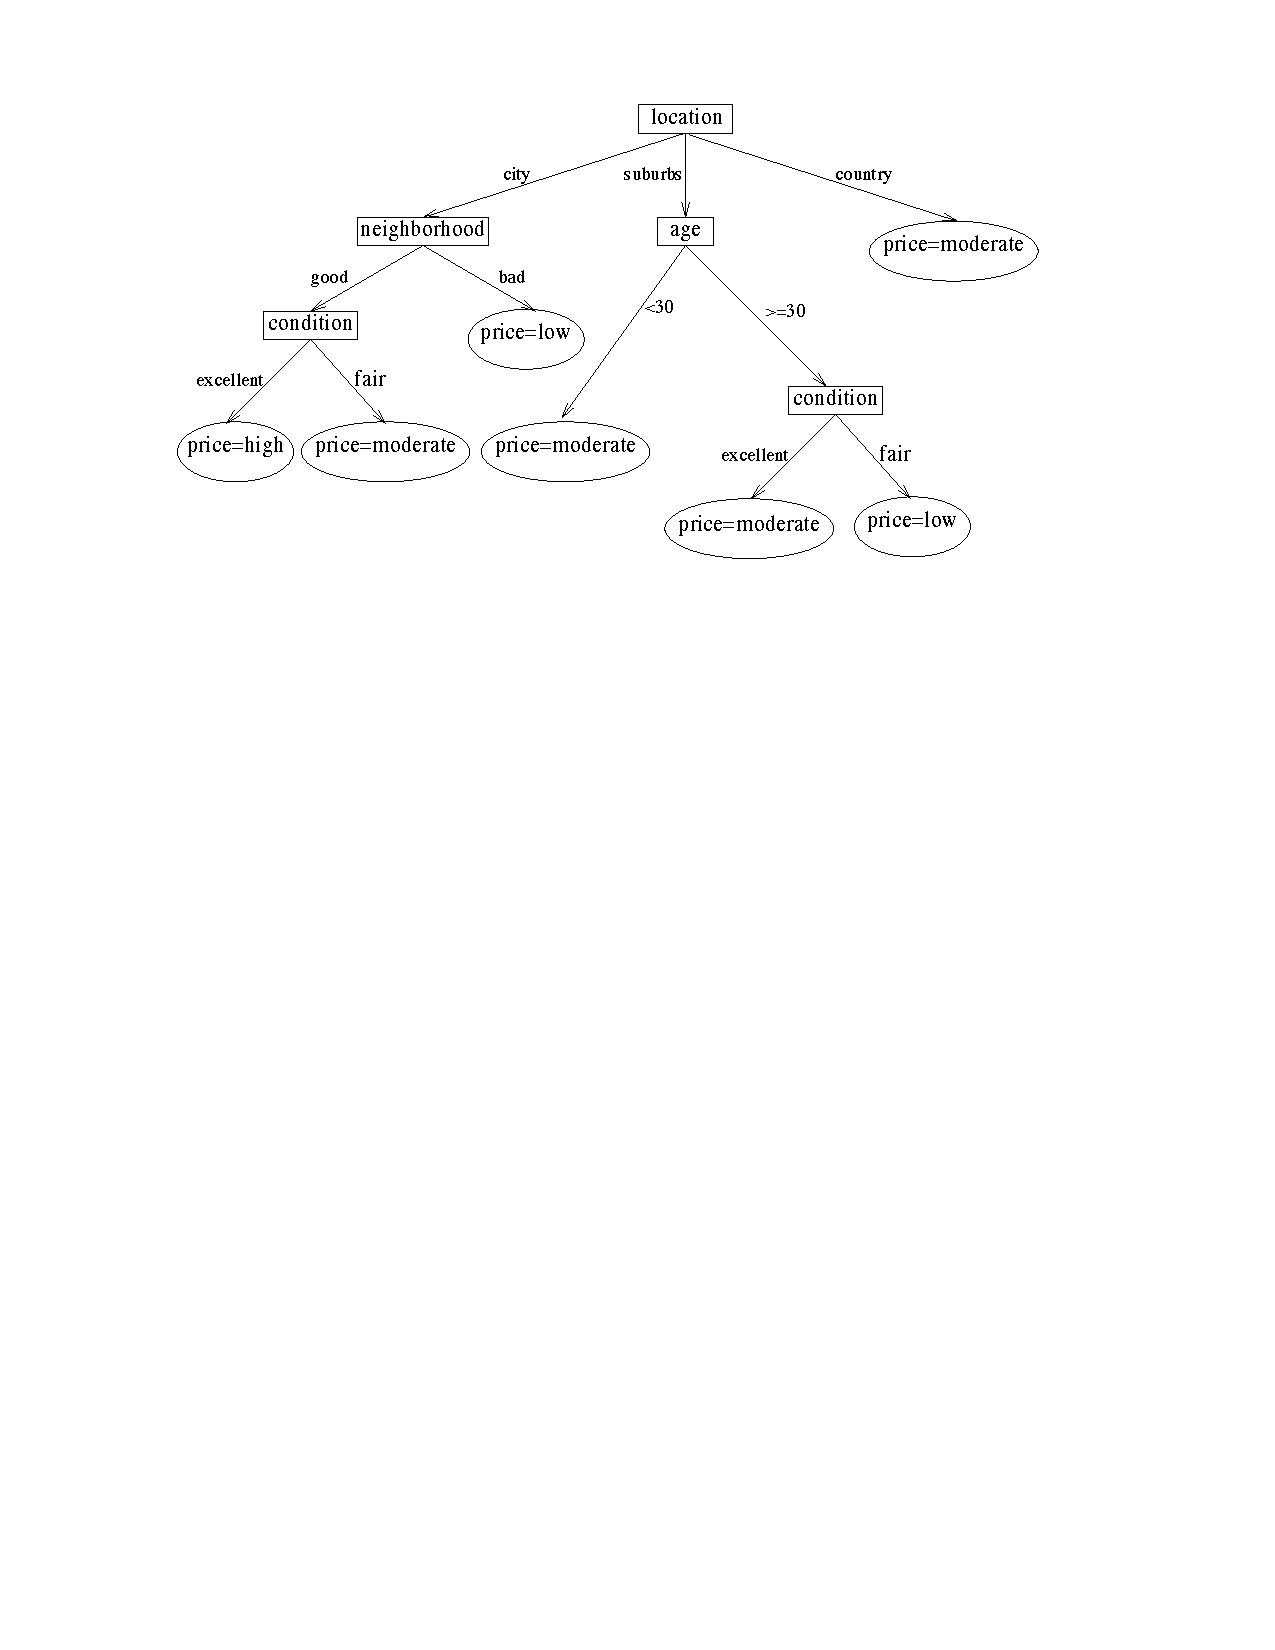
\includegraphics[width=0.86\textwidth]{dt}
    \caption{Example of a decision tree, Rectangles represent internal nodes and ovals represent leaf nodes (possible solution)\cite{KER:70953}}
    \label{fig:dtree}
  \end{center}
\end{figure}

Decision tree classifiers can be used in large datasets with high dimensional data and still be fast and easy to understand its result.
One of its' main advantages due to its white box model of learning, is that at anytime it is possible to understand the reason behind each and every result.
In addition to that, decision tree classifiers are very robust and require no prior knowledge of the domain or parameter settings.

On the other hand, the problem of learning a optimal decision tree is NP-Complete \cite{Hyafil197615}.
Therefore, in practical applications of decision tree learning algorithms, some heuristics need to be used,
usually a greedy algorithm, which can lead
to local optimal decisions being made for each node. The utilization of such algorithms cannot guarantee the global optimal solution to the problem.
There are many algorithms that implement the decision tree principles, such as ID3, C4.5 and CART.

\subsubsection{Random Forests}

Random Forests \cite{raey} are an ensemble learning method for classification and regression, that operates by generating a given number of 
decision trees from a randomly selected uniform subset of the complete training dataset, where the subset distribution is the same across the forest.
After that, at each node the best variable is chosen, using an objective function (similar to what is done in decision trees), and a binary split is done.
This process continues until the trees are fully expanded and there is no pruning of the trees.

Random Forests are robust and fairly able to deal with unbalanced and missing data on the datasets. It is easy to set up with very little configuration
parameters and it also gives good results even if the default parameters are used. The biggest limitation of this algorithm is not being able to
predict beyond the range of the training data when used for regression, because randomly selected inputs give better results in classification than regression \cite{raey}.

\subsubsection{Support Vector Machines}

Support Vector Machine (SVM) is a supervised learning algorithm with great results in pattern recognition.
\cite{Cortes95support-vectornetworks} To achieve this results, SVMs rely on spatial division of classes. The division can be
made without dimensional limit. In other words, the plane or hyperplane that separates the classes can have any number of dimensions. In the figure
~\ref{fig:svm_nonlin} we can see an example of this multidimensional spatial division.

%\cite{citeulike:989242}
\begin{figure}[h]
  \begin{center}
    \leavevmode
    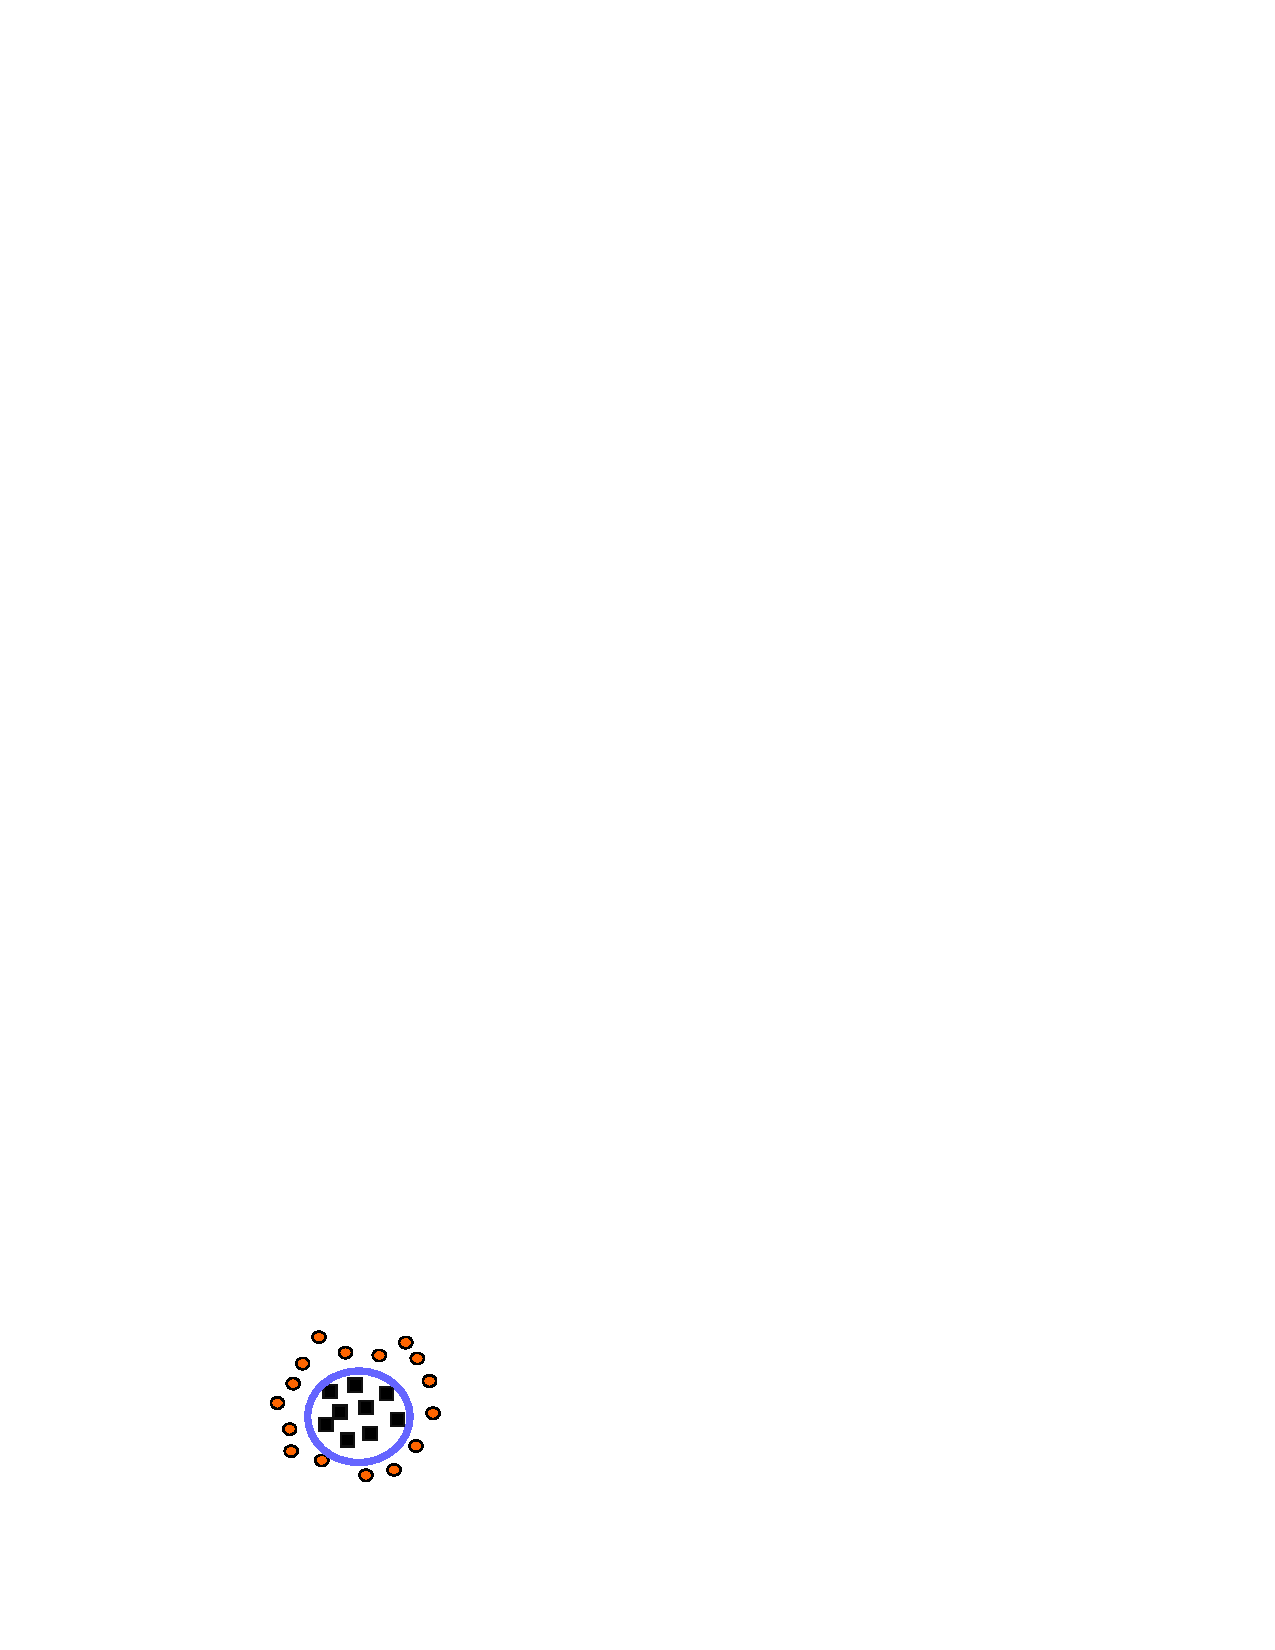
\includegraphics[width=0.66\textwidth]{svm_nl}
    \caption{Example of a non linear separation (quadratic discriminant)\cite{Bennett03supportvector}}
    \label{fig:svm_nonlin}
  \end{center}
\end{figure}

However, the speed of training and testing is low, even for fastest SVMs.
It is also directly limited to two-class tasks\cite{Cortes95support-vectornetworks},
requiring the use of other algorithms to reduce multi-class tasks to binary ones. Although, some work has been done to try to avoid
decomposing the problem in multiple binary class problems.\cite{Crammer:2002:AIM:944790.944813}

In the past few years, this method is also being used to classify internet traffic with excellent results.\cite{Yuan2010}


\subsubsection{KNN}

The \emph{k-nearest-neighbor} algorithm is among the most simple classification algorithms and it has been around since the 1950s \cite[p.348]{HanKam06}.
KNN is a non-parametric method which can be used in classification and regression problems and it is mostly used in the area of pattern recognition.
This algorithm is a type of instance-based learning, or lazy learning, which means that every computation is deferred until classification. By deferring 
computation to classification phase this algorithm is slow at classifying instances. To classify a new instance, the algorithm has to calculate
the \emph{Euclidean distance} between the new instance and every instance in the training set.

Since introduction of this algorithm, some variations of it appeared to help solve the shortcomings of \emph{kNN}.\cite{DBLP:journals/corr/abs-1007-0085}
The more notable are:
\begin{itemize}
\item \textbf{Clustered k nearest neighbor} \cite{journals/jcp/ZhouLX09} is an improved version of k-nn mixed with a clustering algorithm, which allow, for example, 
better performance in classifying text.
\item \textbf{k-d tree nearest neighbor (kdNN)} \cite{Sproull1991} helps to improve, in some cases, the completion time of the classification in logarithmic time.
\item \textbf{Orthogonal Search Tree Nearest Neighbor} \cite{955110} greatly improves efficiency of k-nn, especially for large datasets.
\end{itemize}

\subsection{Clustering Algorithms}\label{sec:clust}

Clustering is the process of grouping similar entries/objects into different groups, in other words, it is the method of breaking a set into various subsets according to some
metric. This groups/subsets are not known from the start and clustering is sometimes considered the most important unsupervised learning problem\cite{DBLP:journals/corr/abs-1205-1117}.

Clustering methods can be divided in\cite{HanKam06}:
\begin{itemize}
\item \textbf{Partitioning Methods} start with an initial number of groups, and reallocates iteratively the elements on the groups
to convergence\cite{DBLP:journals/corr/abs-1205-1117}. Some examples of partitioning methods are based on heuristics like \emph{k-mean algorithm}
and \emph{k-medoids algorithm}.

\item \textbf{Hierarchical Methods} work by grouping data into a tree of clusters\cite{HanKam06}. This methods can be further divided into two
groups: \emph{agglomerative} (bottom-up) and \emph{divisive} (top-down)\cite{DBLP:journals/corr/abs-1205-1117}. At the beginning of an \emph{agglomerative} algorithm,
each object is a cluster and this clusters merge with each other, to form less but larger clusters. The opposite occurs for \emph{divisive} algorithms. The end 
condition for both is a distance threshold.\cite{HanKam06}

\item \textbf{Density-Based Methods} were developed to find clusters with odd forms, relying on the premise that the clusters are located in high density areas
that are separated from each other by low density zones \cite{HanKam06}. Some examples of algorithms which implement this method are \emph{DBSCAN} and \emph{SSN}.

\item \textbf{Grid-Based Methods} uses a multiresolution grid data structure. It divides the object space into a finite number of cells, that
form a grid structure, on which all of the operations for clustering are performed. This approach has a fast processing time,
which is typically independent from the number of data objects but, on other hand, dependent on the number of cells per dimension on the object space\cite{HanKam06}.
Some examples of algorithms which implement the rules of this method are \emph{STING},\emph{WaveCluster} and \emph{CLIQUE}.

\item \textbf{Model-Based Clustering Methods} tries to understand the mathematical rule behind the data, in other words, it is an
''attempt to optimize the fit between the given data and some mathematical model''\cite[p. 429]{HanKam06}. This method assumes 
that the data was generated with some underlying probability. Some examples of this algorithms are \emph{Expectation-Maximization},
\emph{Conceptual Clustering} and \emph{Neural Networks}.

\end{itemize}
%\subsection{Regression Algorithms}\label{sec:regr}

\subsection{Data Mining Tools}
Today there are lots of free tools on the internet which can help us to test and use data mining techniques.
Some of the most used will be presented bellow.

\subsubsection{Weka}

Weka\footnote{ Available at \url{http://www.cs.waikato.ac.nz/~ml/weka/}} is a popular, open source, suite of machine learning software written in Java.
It was created at the University of Waikato, New Zealand in 1997. It has an easy to use and comprehensive GUI with access to an enormous deck of machine learning algorithms.

\begin{figure}[h]
  \begin{center}
    \leavevmode
    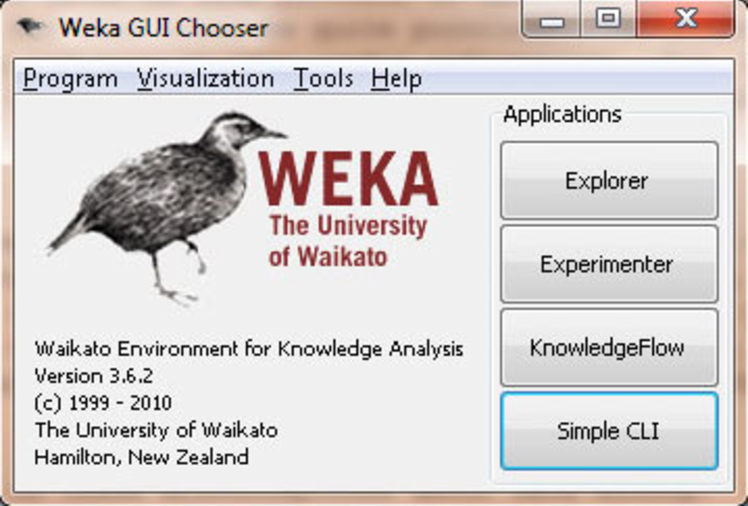
\includegraphics[width=0.66\textwidth]{weka}
    \caption{Screenshot of Weka \url{http://www.ibm.com/developerworks/library/os-weka1/weka-startup1.jpg}}
    \label{fig:RapidMiner}
  \end{center}
\end{figure}


\subsubsection{Apache Mahout}

Apache Mahout\footnote{ Available at \url{http://mahout.apache.org}} is an open source machine learning library to build scalable machine learning libraries.
Its core algorithms are implemented on top of map/reduce paradigm, to help in the scalability of the solution.
Since it is easier to get a cluster of server than an ultra high frequency CPU, and the market trend is to develop many and multi core solution, it is always the best option for processing large quantities of data scalable software.

According to their website, \emph{Mahout} has:
\begin{itemize}

\item User and Item based recommenders
\item Matrix factorization based recommenders
\item K-Means, Fuzzy K-Means clustering
\item Latent Dirichlet Allocation
\item Singular value decomposition
\item Logistic regression based classifier
\item Complementary Naive Bayes classifier
\item Random forest decision tree based classifier
\item High performance java collections (previously colt collections)
\item  A vibrant community

\end{itemize}

\subsubsection{RapidMiner}

Rapid Miner\footnote{ Available at \url{http://www.rapidminer.com/}} is a complete solution for data mining problems. It is available in a form of
a standalone GUI application.
\begin{figure}[h]
  \begin{center}
    \leavevmode
    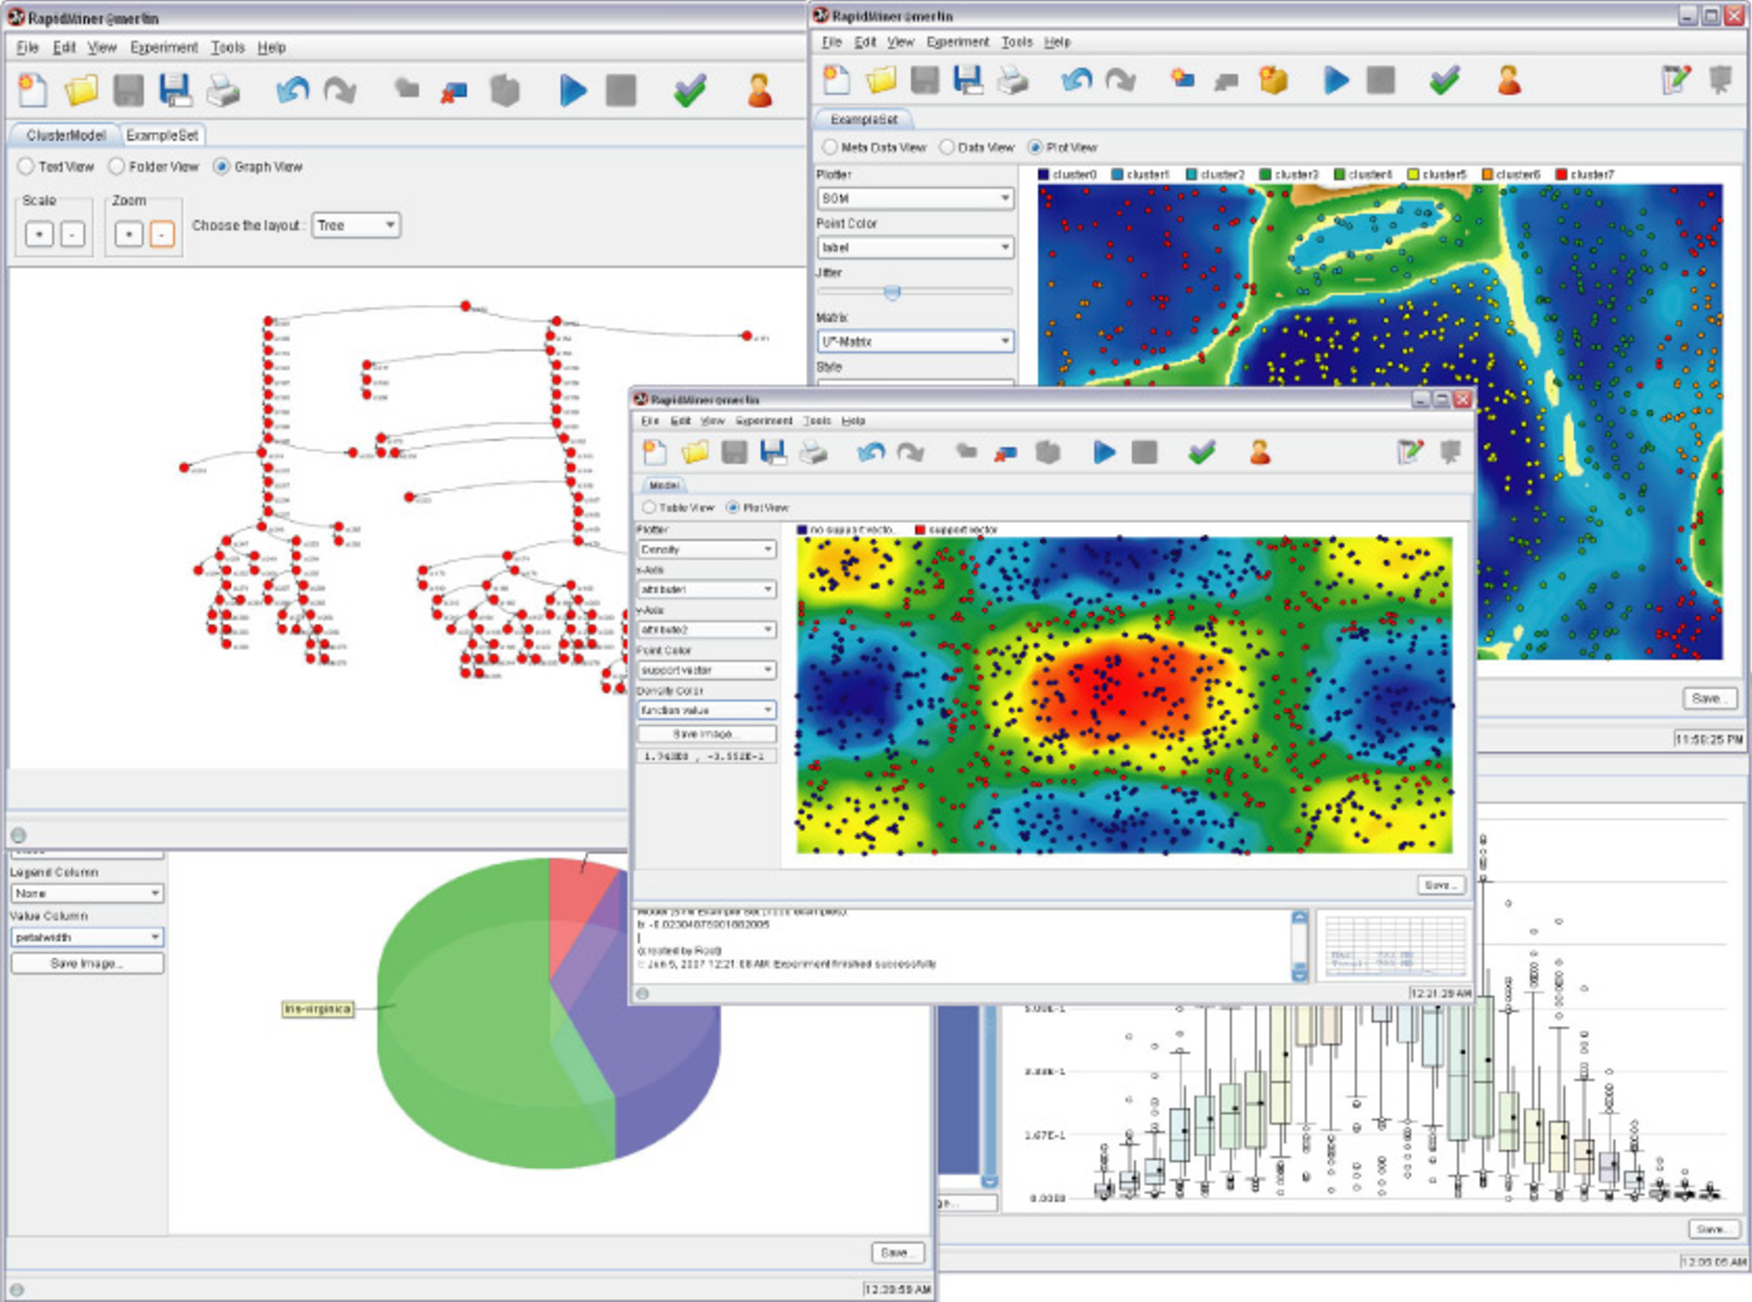
\includegraphics[width=0.66\textwidth]{rapidminer}
    \caption{Screenshot of RapidMiner \url{http://mloss.org/media/screenshot_archive/rapidminer_collection.jpg}}
    \label{fig:RapidMiner}
  \end{center}
\end{figure}

 Although it is a commercial product, there is also a free tier, and the core and earliest versions are open source. This application
is one of the main players of this market and it is easily expandable through plug-ins available online.

\subsubsection{R Language}
R\footnote{ Available at \url{http://www.r-project.org}} is a free programming language and software environment for graphics generation and statistical computing.
Developed by Ross Ihaka and Robert Gentleman at the University of Auckland, New Zealand, in 1993 \cite{Ihaka98r:past}, it is still in active development and
greatly used by statistics and data miners.

R is an implementation of S, the statistics programming language, and it uses some characteristics inspired on Scheme.
R is a GNU tool, so it is completely free. There are wrappers to almost every language which can be used to access R variables from other programming languages.


\section{Web Usage Mining}\label{sec:network}

The main area which this project focus on the utilization of ad requests logs
to predict future requests of the users. This is analogous to work
which have been done in the area of user future requests prediction.
Next it will be done a little overview of what have been studying in the area of web
usage data mining, in the last years, in order to identify possible approaches
to solve the problem of this thesis.


%\subsection{Instance-based regression algorithms}\label{sec:instance}
